\subsection{Příčkové LC filtry}\label{s:LC}
Pasivní dolní propust je realizována zapojením induktoru ke vstupnímu napětí a k~této větvi je následně zapojen paralelně rezistor. Pasivní horní propust má ke vstupu připojený sériově rezistor a poté k~této větvi paralelně induktor. \\
\\
K realizaci filtrů vyšších řádů se užívají $\pi$ nebo T~články s LC prvky. Podle Vedrala a Svatoše \cite{8} musí být při návrhu filtru zohledněn vnitřní odpor zdroje $R_s$ a zatěžovací odpor $R_L$. LC filtry jsou tedy dvojitě zakončeny. Indukčnosti a kapacity prvků se určí z rovnic pro normované kapacity a indukčnosti. Normované hodnoty budou vypočteny pro mezní kmitočet $\omega _0 = 1/\sqrt{LC}$ a pro zatěžovací odpor $R_L$. Hodnoty prvků lze pro požadovanou aproximaci odečíst z tabulek. Pro LC filtry se používá kmitočtová oblast $10^{3}$\,Hz--$10^{2}$\,MHz.\\
\\
\begin{figure}[h]
\centering
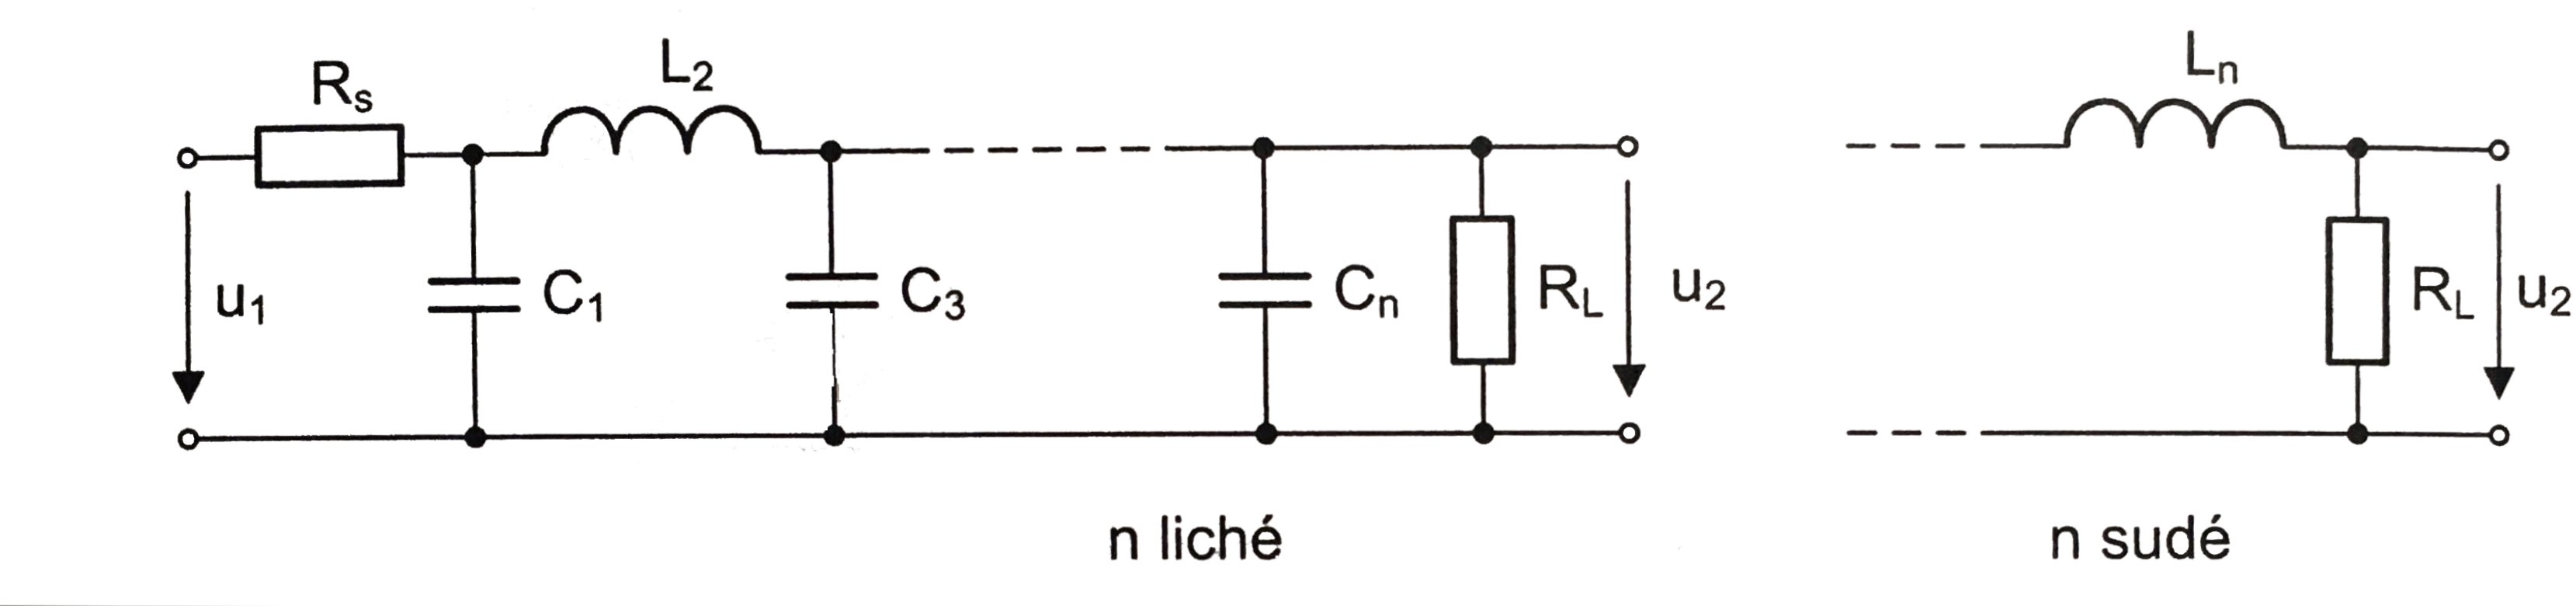
\includegraphics[scale=0.125]{piclanky.png}
\caption[Pasivní dolní propust n-tého řády s $\pi$ články]{Pasivní dolní propust n-tého řády s $\pi$ články \cite{8}}
\end{figure}
\begin{figure}[h]
\centering
\includegraphics[scale=0.078]{tclanky.png}
\caption[Pasivní dolní propust n-tého řády s T články]{Pasivní dolní propust n-tého řády s T články \cite{8}}
\end{figure}
\subsection{Gyrátory}\label{s:GYR}
\noindent K převodu induktoru na zapojení s kapacitorem byla použita struktura označovaná jako gyrátor. Jde o náhradu původního obvodu s induktorem vhodným uspořádáním rezistorů a kapacitorů tak, že výsledná impedance vypadá jako induktor. Jelikož po této substituci v obvodu zůstanou jen R,C prvky, jedná se o ARC syntézu. \\
\\
 Gyrátor je podle Martinka, Boreše a Hospodky \cite{12} typ invertoru. Pro invertory platí, že jejich vstupní impedanci lze napsat ve tvaru\begin{equation}
Z_{vst} = \frac{a_{12}}{a_{21}}\frac{1}{Z_L} = \frac{a_{12}}{a_{21}}Y_L.
\end{equation}
Pokud jsou parametry $a_{12}, a_{21}$ reálné a kladné, hovoříme o gyrátoru. Symbol gyrátoru je na obrázku~\ref{s:G}. Gyrátor se nejúspěšněji dá realizovat paralelním spojením dvou napětím řízených zdrojů proudu s opačným znaménkem. Zapojení s OTA odpovídá dvěma zesilovačům, jeden s uzemněnou zápornou a druhý s uzemněnou kladnou svorkou vstupu. Výstup prvního ze zesilovačů je propojen s volnou vstupní svorkou druhého a naopak.
\begin{figure}[h]
\centering
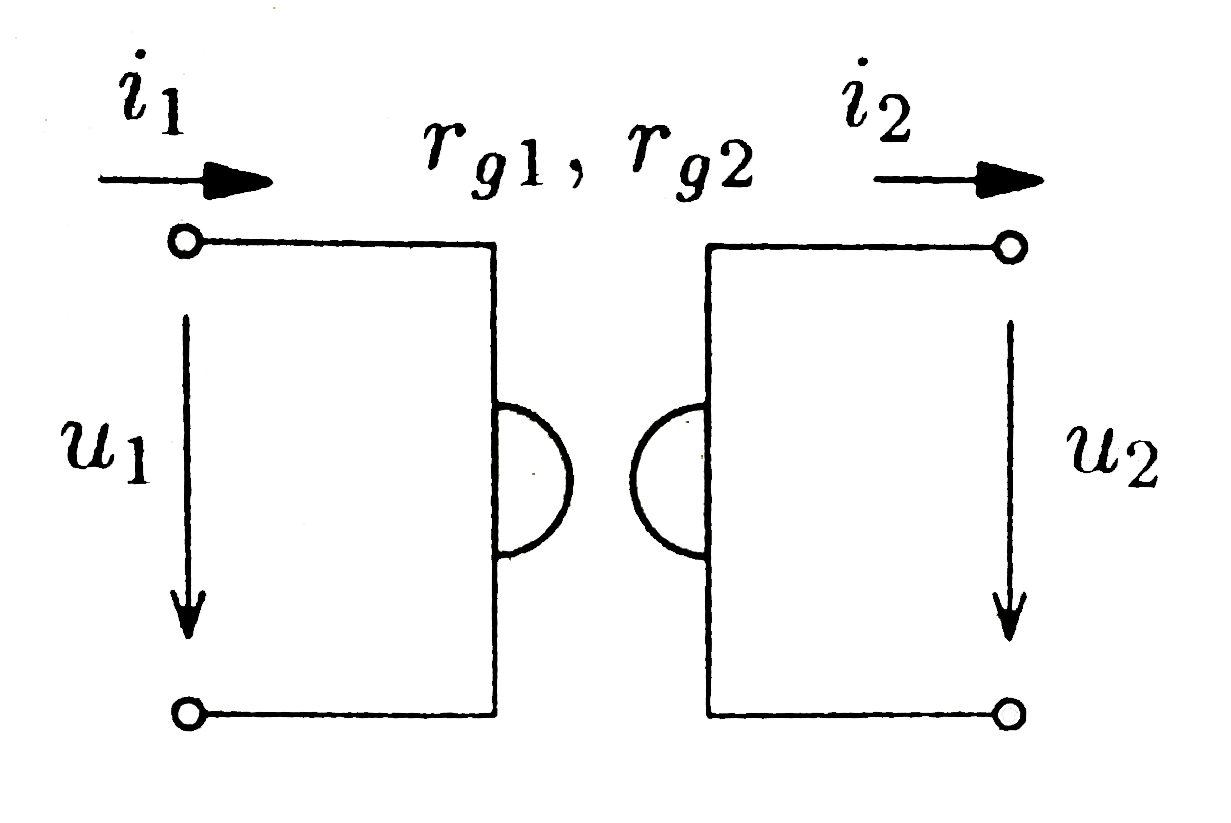
\includegraphics[scale=0.095]{gyr.png}
\caption{Definice gyrátoru \label{s:G}}
\end{figure}
Podle Schaumanna a Valkenburga \cite{13} nelze gyrátor dobře realizovat s obyčejnými operačními zesilovači, běžně se používají \textit{General Impedance Converters} (GIC). Převod induktoru na jiné zapojení s ekvivalentní impedancí má praktické využití v integrovaných obvodech, kde jsou kapacitory preferovány nad induktory kvůli malým rozměrům. Navíc se induktory musí složitě vyrábět na danou hodnotu. V návrhu integrovaných obvodů se také většinou nepoužívají rezistory kvůli místu na čipu, které zabírají. \\
\\
Gyrátor je principielně spojení invertujícího a neinvertujícího napětím řízeného zdroje proudu, a proto ho lze realizovat snadno s transkonduktančními zesilovači. Na obrázku~\ref{s:GO} jsou podle Schaumanna a Valkenburga \cite{13} znázorněny dva gyrátory s kapacitorem. 
\begin{figure}[h]
\centering
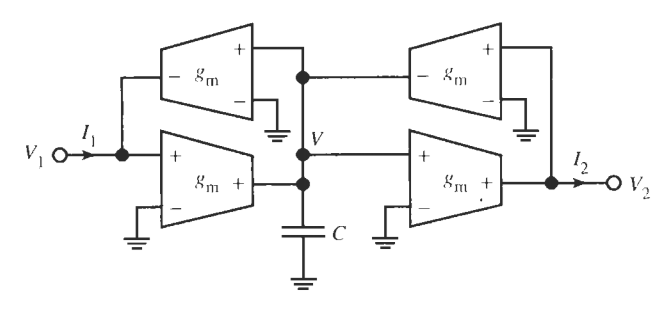
\includegraphics[scale=0.4]{gyrator.png}
\caption[Plovoucí induktor realizovaný kapacitorem a dvěma gyrátory]{Plovoucí induktor realizovaný kapacitorem a dvěma gyrátory \label{s:GO}}
\end{figure}
Obvodovou analýzou v uzlu $V$ byla obdržena rovnice
\begin{align}
pCU &= g_mU_1 - g_mU_2
\end{align}
a dva proudy na výstupu
\begin{align}
I_1 = I_2 = g_mU.
\end{align}
Zkombinování rovnic a eliminace V vede k rovnici plovoucího induktoru mezi napětími $U_1$ a $U_2$.
\begin{align}
I_1 = I_2 = \frac{g_m^2}{pC}(U_1 - U_2) = \frac{1}{pL}(U_1 - U_2)
\end{align}
Z rovnice lze snadno odvodit, že kapacita kondenzátoru použitého jako náhrada zapojení induktoru v zapojení s OTA je rovna $C_L = L g_m ^2$. \\
\subsection{Vliv zátěže na funkci obvodu}
\noindent V simulaci se samozřejmě předpokládá, že všechny OTA zesilovače jsou ideální. Chování filtru ve výsledku ovlivní nedokonalosti reálných OTA (ztráty, parazitní chyby). Další nevýhodou jsou kondenzátory a jejich odchylka od jmenovité hodnoty --- oproti tomu rezistory mají obecně minimální odchylku od jmenovité hodnoty. Z literatury podle Schaumanna a Valkenburga \cite{13} také víme, že reálné transkonduktance nejsou idální zdroje proudu (s nulovou výstupní admitancí) a že většina $g_m$-C bloků použitých v obvodu má nenulové výstupní admitance. Jejich chování bude tedy extrémně závislé na zátěži, což může úplně změnit zamýšlenou funkci obvodu. Například ve~sčítacím obvodu na obrázku \ref{s:BLO}, popsaným rovnicí \ref{s:BLO3}, zátěžová admitance $Y_L$ změní $g_{m3}$ na $g_{m3} + Y_L$. Podobně zátěž $Y_L$ na ztrátovém integrátoru na obrázku \ref{s:OTA-INT} (popsaný rovnicí \ref{s:OTA-INT1}) způsobí změnu $g_m$ na $g_m + Y_L$ v přenosové funkci integrátoru. Proto by transkonduktanční obvody obecně měly být navrženy tak, aby základní bloky řídily vysoko-impedanční uzly (např. vstupy jiných OTA). Pokud mají být řízeny velké zátěže, obvod s OTA musí být řízen \textit{bufferem} (v~pinoutu LM13700 na obrázku \ref{s:PIN} pin 7, 8 pro první OTA zesilovač a 9,10 pro druhý OTA zesilovač). Případně lze jako \textit{buffer} použít operační zesilovač s jednotkovým zesílením.\\
\\
\noindent K určení chování obvodu musíme mít podle Schaumanna a Valkenburga \cite{13} na paměti, že parazitní admitance $y_p = y_i + y_o$ je přítomna na každém uzlu spojujícím dva OTA zesilovače. Pokud pro jednoduchost předpokládáme, že všechny OTA jsou stejné a výstup $V_{out}$ je zatížen $Y_L$, dostaneme vztah
\begin{equation}
V_{out} = \frac{g_{m1}}{y_p}\frac{g_{m2}}{y_p}\frac{g_{m3}}{y_p} \ldots \frac{g_{mn}}{Y_L + y_p}(V_{in} - V_{out}).
\end{equation}
\noindent Po úpravě
\begin{align}
\frac{V_{out}}{V_{in}} &= \frac{1}{1 + (\frac{y_p}{g_m})^n(1 + \frac{Y_L}{y_p})} \simeq 1,\\
\lvert \frac{y_p}{g_m} \rvert ^n &\ll 1.
\end{align}
\noindent Podobně pro výstupní impedanci $Z_{out}(p)$ platí
\begin{align}
Z_{out}(p) &= \frac{\frac{1}{y_p}}{1 + (\frac{g_m}{y_p})^n} \simeq \frac{1}{y_p}(\frac{y_p}{g_m})^n,\\
\lvert \frac{y_p}{g_m} \rvert ^n &\ll 1.
\end{align}
\noindent Navrhnout transkonduktance tak, aby platilo $g_m \gg \lvert y_p \rvert$, $\lvert V_{out}/V_{in} \rvert  \simeq 1$ a $\lvert Z_{out} \rvert \simeq \lvert 1/y_p \rvert$ pro dostatečně velká n, je poměrně snadné. Obvykle se volí $n = 2$ nebo $n = 3$.
\subsection{Ladění filtru}
\noindent Pokud se analogový filtr má chovat podle specifikací, musí být navržen s přesnými hodnotami komponent. Podle Schaumanna a Valkenburga \cite{13} přenosová funkce závisí na frekvencích nul a pólů, Q faktoru pólů (Q faktor definuje, jak moc je systém podtlumený), zesílení --- tyto parametry zase závisí na přesné hodnotě součástek. Kritické frekvence s jednotkami 1/čas jsou určeny absolutními hodnotami kapacitorů a rezistorů. Zesílení a Q faktor je určen poměrem kapacitorů a rezistorů. V diskrétních obvodech můžou být problémy vyřešeny laděním, buď před, nebo po dokončení návrhu. Pokud například máme časovou konstantu $T = RC$, můžeme změřit T a přizpůsobit rezistor (trimmerem), dokud neobdržíme požadovanou časovou konstantu $T_0$.\\
\\
Hlavním problémem ladění je přesné nalezení časové konstanty $C_U/g_m$, která mění mezní kmitočet. Časovou konstanta může být obdržena změnou $g_m$. Pokud je zesílení integrátoru jednotkové, časová konstanta bude nastavena na $1/\omega _{ref}$. Pokud bude referenční signál poslán na vstup integrátoru a oba vstupní a výstupní signály přes dva indentické špičkové detektory, naladíme $g_m$ dokud jednotkové zesílení frekvence integrátoru nebude~$f_{ref}$. Tomuto zapojení se říká \textit{Master-Slave Tuning}. Také lze použít ladění pomocí Q-faktoru. \\
\\
Dalšími problémy obecně u OTA, které mohou ovlivnit funkci obvodu, je nízké stejnosměrné zesílení, nízké UGBW a vysoký šum. Tyto problémy se dají částečně vyřešit zvýšením transkonduktance. Zvýšením výstupní impedance se zvýší i stejnosměrné zesílení.
\subsection{Zhodnocení funkčnosti}
\noindent Pro návrh filtru ve spojitém časovém  pásmu se pro zhodnocení funkčnosti používá THD (\textit{Total Harmonic Distortion}) a SNR (\textit{Signal-to-Noise Ratio}). SNR lze definovat jako poměr mezi přijatým signálem a šumem spojeným se získáním tohoto signálu. Hodnota SNR roste s rostoucí velikostí signálu. Maximální hodnoty SNR je dosaženo při zaznamenání maximálního signálu (tzn. při dosažení úrovně saturace) \cite{21}. Poměr větší než 1 (0\,dB) znamená, že amplituda signálu je větší než šumu. Definice je podle \cite{22}
\begin{equation}
SNR_{dB} = 10 \cdot log_{10}\left(\frac{P_{signal}}{P_{noise}}\right).
\end{equation}
 Hlavní vliv na THD má linearita transkonduktance, protože do systému filtru indukuje harmonické zkreslení (HD --- \textit{Harmonic Distortion}). Pro nízké frekvence má na SNR vliv tepelný šum --- ten může vzniknout vlivem nerovnoměrností struktury, teplotními kmity krystalové mřížky náhodným, či tepelným pohybem nabitých částic (zpravidla elektronů) v rámci elektrických vodičů. Teoreticky se dá říci, že tepelný šum není generován jen ve vodičích, jejichž teplota je rovna nebo téměř rovná absolutní nule. Jakákoliv vyšší teplota již znamená náhodný pohyb elektronů a tedy vznik šumu (Motchenbacher \cite{23}, \cite{24}). Vliv tepelného šumu ovlivňuje hlavně funkčnost OTA s menšími hodnotami transkonduktance. Tepelný šum je také znám jako 1/f šum, protože jeho spektrální hustota výkonu je inverzní k frekvenci \cite{1}. Ztráty způsobené šumem mohou být vzhledem ke konečnému zesílení kompenzovány předzesilovačem. \\
\\
Některá zapojení s nekonečnou vstupní imepedancí mají poměrně vysokou výstupní impedanci. Kaskádní zapojení lze rovněž kompenzovat \textit{bufferem}, což ale sníží šířku pásma celé struktury.\\